\section{Data and methods}
\label{sec:methods}
\subsection{Target and interpretation}
Let $C_t$ denote a daily closing price and define
\begin{equation}
r_t=\log(C_t/C_{t-1}),\qquad RV_t=r_t^2,\qquad
 y_{t+1}=\log(RV_{t+1}+\varepsilon),\quad\varepsilon=10^{-8}.
\end{equation}
The notation $RV_t$ follows the project code; it is a daily squared return, not a sum of intraday squared returns. Its conditional expectation is a conditional second moment, equal to conditional variance only when the conditional mean return is zero. Forecasts are mapped back by
\begin{equation}
\widehat{RV}_{t+1|t}=\max\{\exp(\widehat y_{t+1|t})-\varepsilon,10^{-12}\}.
\end{equation}
A model minimizing squared error in the log target estimates a different functional from one modeling conditional variance directly. By Jensen's inequality, exponentiating a conditional mean of the log target does not generally recover the conditional mean of the untransformed target. Consequently, disagreement between log-MSE and QLIKE rankings need not imply an implementation error.

\subsection{Inputs, sample construction, and data audit}
The study uses daily CSI300, SSE50, and Nasdaq market records, monthly Chinese EPU for the Chinese indices, and monthly US EPU for Nasdaq. The Chinese series is the mainland-newspaper measure cited in \citet{DavisLiuSheng2019}, rather than an interchangeable substitute for every published Chinese EPU series. Its newspaper sources include the People's Daily and Guangming Daily. The original EPU download versions, release timestamps, and revision histories are not fully archived. Lagging monthly observations reduces contemporaneous overlap but cannot establish a genuine real-time information set.

The CSI300 descriptive sample spans January 2010 to March 2026. Its 3942 prices yield 3941 returns. An archived descriptive output instead contained 3942 returns. Inserting an additional zero between the observations dated 2018-06-15 and 2018-06-19 reproduces 24 historical statistical fingerprints; the historical operation that created that extra observation remains unknown. This insertion is a forensic diagnostic only and is not used for current descriptive statistics or model estimation. The reconciled CSI300 model matrix has 3919 rows without that added zero.

For SSE50, a confirmed holiday record dated 2018-06-18 had zero volume and an unchanged close. Removing that row only after target construction would leave an artificial $\log(10^{-8})$ target on the preceding retained observation. The current pipeline removes the confirmed holiday before constructing returns, features, and targets, consistent with the Shanghai Stock Exchange's 2018 holiday schedule announced on 2017-12-22. Zero volume alone is not used to classify all other dates as holidays. This correction is not a complete audit of every market's calendar or upstream data source.

\begin{table}[htbp]\centering
\caption{Current chronological sample definitions. Dates identify forecast origins.}
\begin{tabular}{lrrrr}\toprule
Market & Prepared & Initial train & Validation & Test\\\midrule
CSI300 & 3919 & 1500 & 500 & 1919\\
SSE50, corrected & 3919 & 1500 & 500 & 1919\\
Nasdaq & 4054 & 2000 & 500 & 1554\\\bottomrule
\end{tabular}
\begin{flushleft}\small CSI300 and corrected SSE50 test origins: 2018-05-03 to 2026-03-30. Nasdaq: 2020-01-23 to 2026-03-30. Historical SSE50 had 3915 prepared rows and 1915 test rows. These counts describe the recorded inputs, not a requirement for arbitrary new data.\end{flushleft}
\label{tab:samples}
\end{table}

The original archived model matrices were reconciled by dates, features, 24 EPU lags, targets, and sample flags. Matching an archive establishes provenance consistency, not that all upstream observations are error-free. Current descriptive statistics and diagnostics use the corrected 3941-return series (Tables~\ref{tab:desc_return_short} and~\ref{tab:diagnostic_tests_short}). The sample exhibits heavy tails and dependence in squared returns, motivating volatility models without establishing any particular specification as correct.

\begin{table}[htbp]\centering
\caption{CSI300 daily log-return descriptive statistics.}
\label{tab:desc_return_short}
\begin{tabular}{lr}\toprule Statistic & Value\\\midrule
Observations & 3941\\
Mean & $5.8396\times10^{-5}$\\
Standard deviation & 0.013639\\
Minimum & $-0.091544$\\
Maximum & 0.081420\\
Skewness & $-0.576130$\\
Excess kurtosis & 5.460548\\\bottomrule
\end{tabular}
\end{table}
\begin{table}[htbp]\centering
\caption{Distributional and dependence diagnostics for CSI300 returns.}
\label{tab:diagnostic_tests_short}
\begin{tabular}{lrr}\toprule Test & Statistic & $p$-value\\\midrule
Jarque--Bera & 5099.01 & $<0.0001$\\
Ljung--Box, returns, 10 lags & 32.75 & 0.0003\\
Ljung--Box, returns, 20 lags & 64.45 & $1.43\times10^{-6}$\\
Ljung--Box, squared returns, 10 lags & 1051.71 & $1.35\times10^{-219}$\\
Ljung--Box, squared returns, 20 lags & 1526.13 & $9.87\times10^{-312}$\\
ARCH LM, 10 lags & 452.36 & $6.56\times10^{-91}$\\
ARCH $F$, 10 lags & 50.98 & $9.52\times10^{-97}$\\\bottomrule
\end{tabular}
\end{table}
\begin{figure}[htbp]\centering
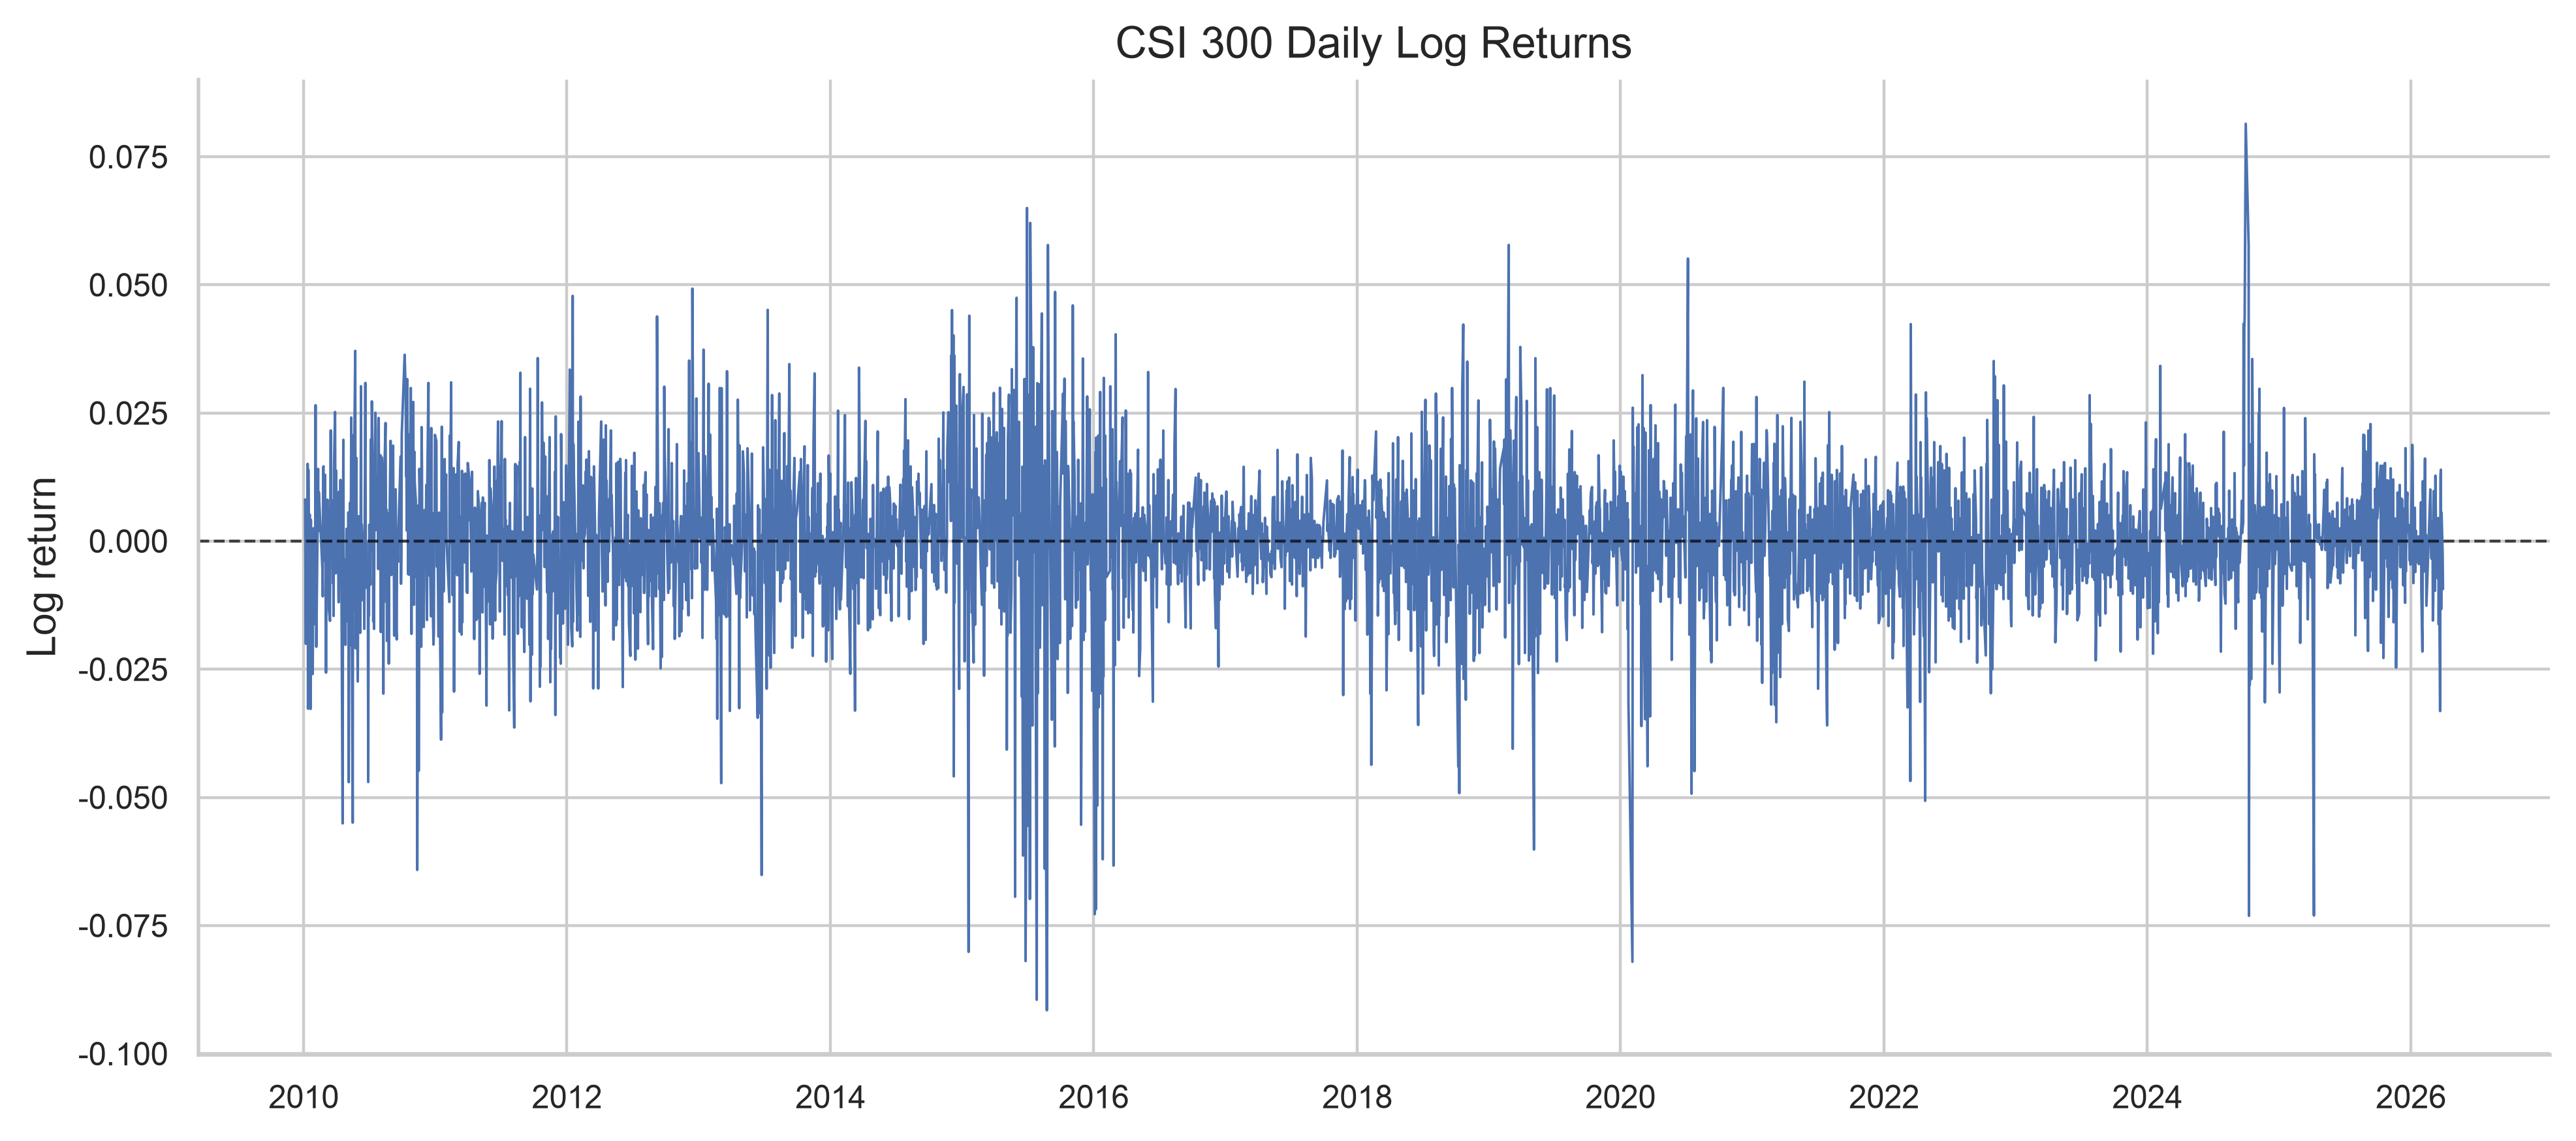
\includegraphics[width=.94\textwidth]{../../results/descriptive-corrected/figure_1_log_return_series.png}\\[0.5em]
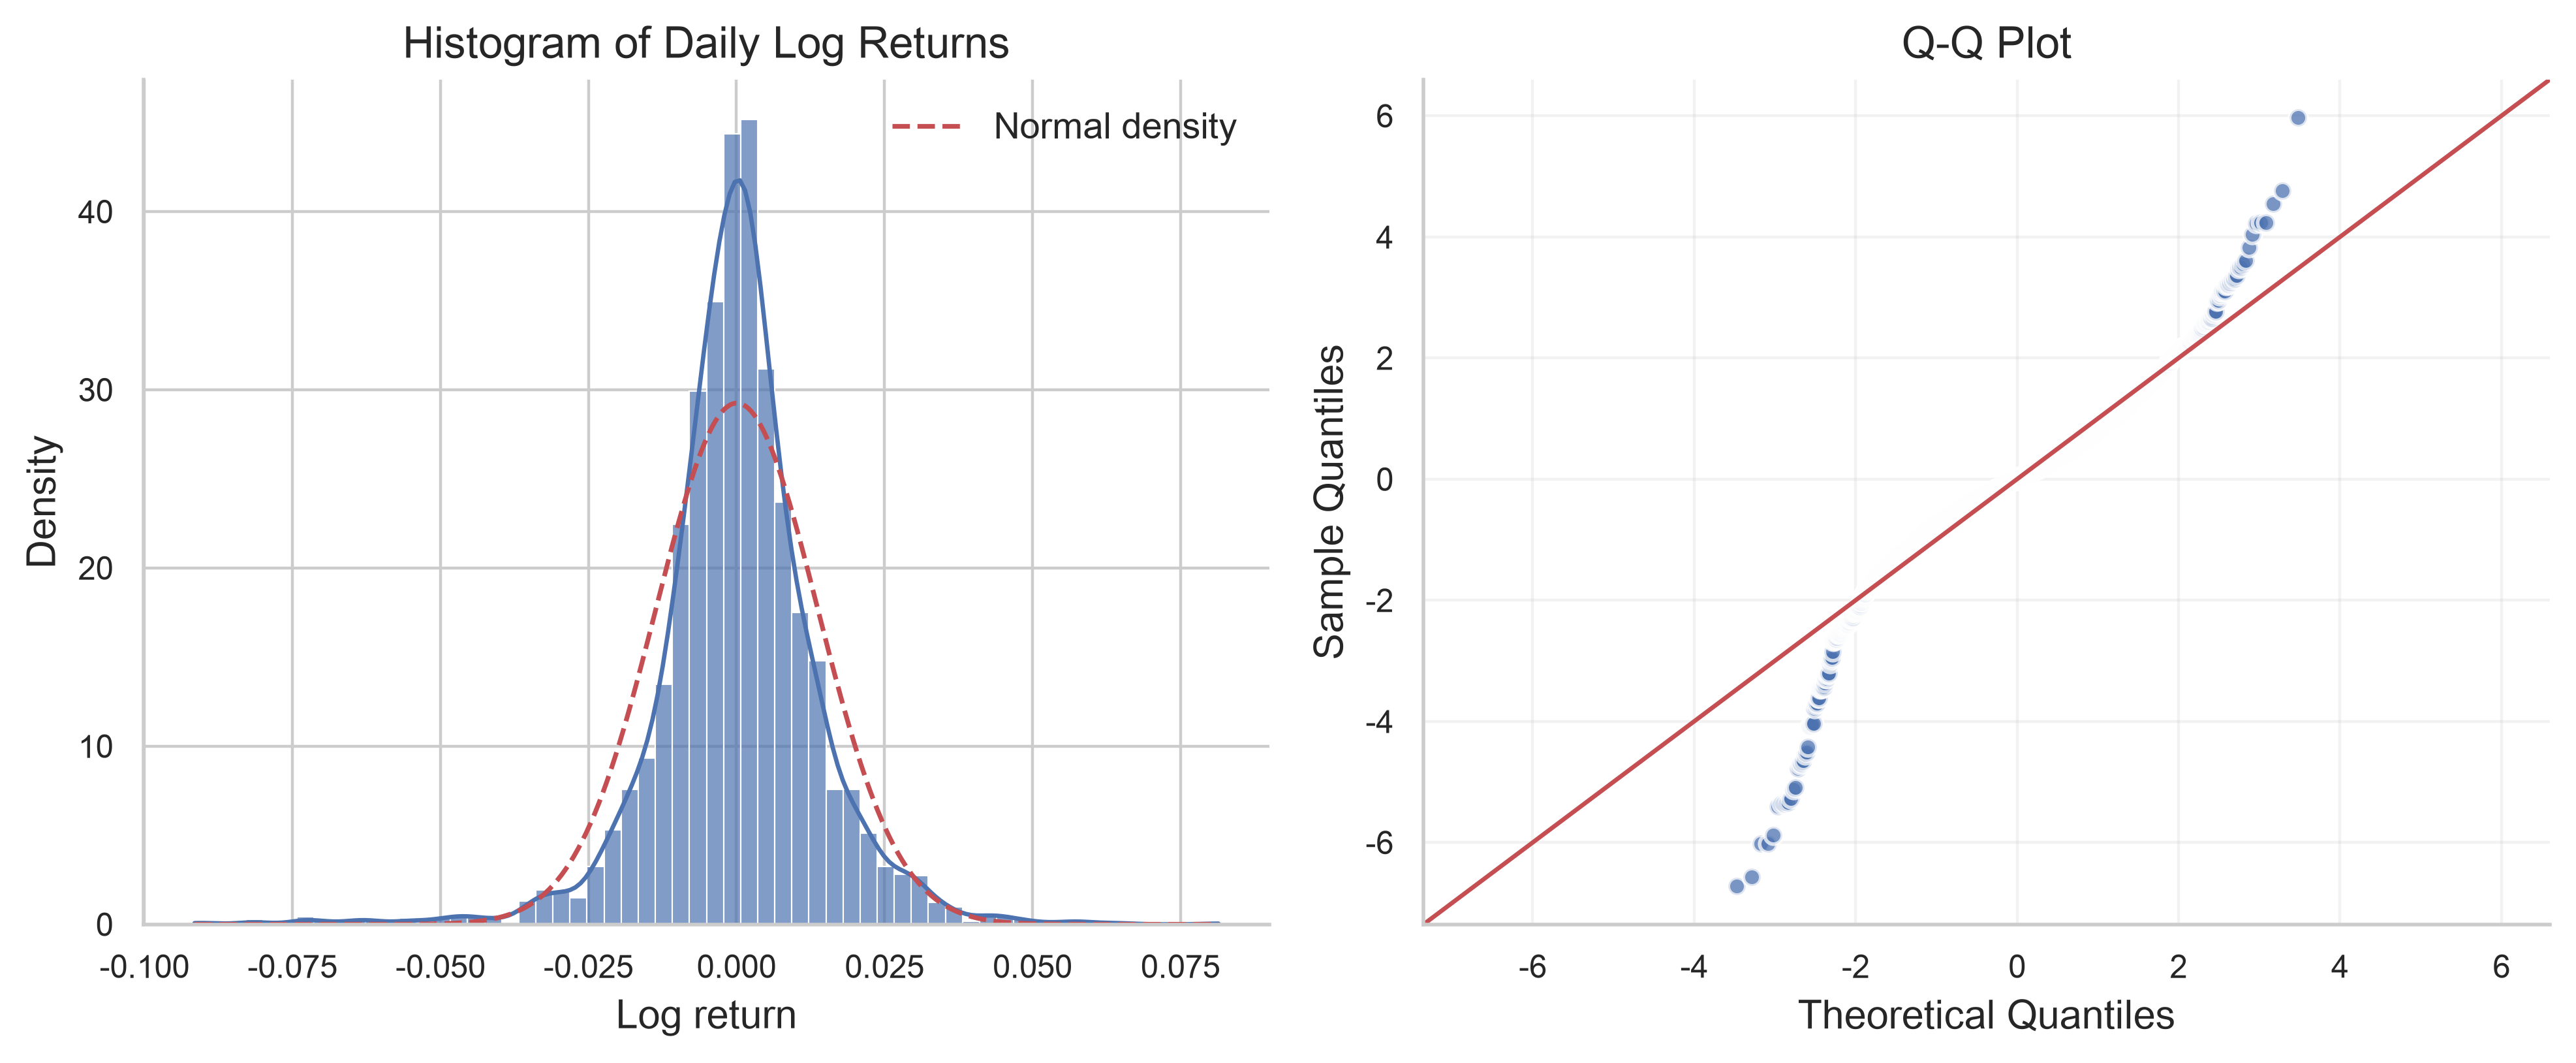
\includegraphics[width=.94\textwidth]{../../results/descriptive-corrected/figure_2_histogram_qq.png}
\caption{Corrected CSI300 return series, distribution, and normal quantile comparison.}
\label{fig:return_ts_qq}
\end{figure}

\subsection{Market-only baselines}
The HAR-style regression is estimated by ordinary least squares:
\begin{equation}
y_{t+1}=\beta_0+\beta_d\log(RV_t+\varepsilon)
+\beta_w\log(\overline{RV}_{t,5}+\varepsilon)
+\beta_m\log(\overline{RV}_{t,22}+\varepsilon)+u_{t+1},
\end{equation}
where $\overline{RV}_{t,h}=h^{-1}\sum_{j=0}^{h-1}RV_{t-j}$. This uses multiscale persistence but not intraday realized variance.

The GARCH benchmark has a zero conditional mean and standardized Student-$t$ innovations:
\begin{equation}
r_t=\epsilon_t=\sqrt{h_t}z_t,\qquad
h_t=\omega+\alpha\epsilon_{t-1}^2+\beta h_{t-1}.
\end{equation}
Under the usual nonnegative parameter restrictions, $\alpha+\beta<1$ is the familiar finite-second-moment stationarity condition. The forecast enters the log-target comparison as $\log(\widehat h_{t+1|t}+\varepsilon)$. EGARCH, GJR-GARCH, and realized-volatility extensions are not included, so this is a limited benchmark comparison.

XGB-Market uses nine predictors in the fixed order shown in Table~\ref{tab:variables_main}. It is fitted to the log target. No winsorization, standardization, or early stopping is used in the matched historical configuration. Important parameters are 300 trees, depth 4, learning rate 0.05, minimum child weight 3, row and column sampling fractions 0.8, $L_1$ regularization 0.1, and $L_2$ regularization 1. The CPU histogram algorithm, 256 bins, and seed 2026 are fixed. Appendix~\ref{app:training} provides the numerical reproduction qualifications.

\begin{table}[htbp]\centering\small
\caption{XGB-Market predictors, in matrix order. $H_t$, $L_t$, and $V_t$ are daily high, low, and volume.}
\label{tab:variables_main}
\begin{tabularx}{\textwidth}{lX}\toprule Code name & Definition\\\midrule
\texttt{log\_rv1} & $\log(RV_t+\varepsilon)$\\
\texttt{log\_rv5} & $\log(\overline{RV}_{t,5}+\varepsilon)$\\
\texttt{log\_rv22} & $\log(\overline{RV}_{t,22}+\varepsilon)$\\
\texttt{ret\_pos} & $\max(r_t,0)$\\
\texttt{ret\_neg} & $\min(r_t,0)$\\
\texttt{range\_log} & $\log(H_t/L_t)$\\
\texttt{range\_log\_5} & Five-observation average of $\log(H/L)$\\
\texttt{log\_volume} & $\log(V_t)$\\
\texttt{dlog\_volume} & $\log(V_t)-\log(V_{t-1})$\\\bottomrule
\end{tabularx}
\end{table}

HAR, GARCH, and XGBoost are re-estimated every 20 retained observations using expanding histories. The phrase ``every 20'' is a refit frequency, not a fixed rolling training-window length or a calendar-day interval. At an origin after the daily close, all target observations used for training must already have been realized. Filtering can make adjacent retained rows differ from adjacent exchange trading days; the timing audit therefore distinguishes row order from actual dates.

\subsection{MIDAS signal and dynamic error correction}
Let $m(t)$ be the calendar month containing forecast origin $t$. The EPU signal uses the preceding $K$ months:
\begin{equation}
s_t(\theta)=\sum_{k=1}^{K}w_k(\theta)\log(EPU_{m(t)-k}),
\qquad w_k\geq0,\quad\sum_{k=1}^K w_k=1.
\end{equation}
This convention excludes the current calendar month's value, but without vintage data it remains a retrospective lag convention rather than verified real-time availability.

For Beta weights, set $x_k=(K-k+1)/(K+1)$ and use
\begin{equation}
a_k=\max\{x_k^{\theta_1-1}(1-x_k)^{\theta_2-1},10^{-12}\},
\qquad w_k=a_k/\textstyle\sum_j a_j.
\end{equation}
For exponential Almon weights, set $z_k=(K-k+1)/K$ and use
\begin{equation}
w_k=\frac{\exp(\theta_1z_k+\theta_2z_k^2)}
{\sum_j\exp(\theta_1z_j+\theta_2z_j^2)}.
\end{equation}
The definitions and orientation of the lag index are part of the specification; a differently ordered lag vector would describe a different signal.

Define the realized first-stage forecast error as $e_t=y_t-\widehat y^{\mathrm{XGB}}_{t|t-1}$. These are sequential forecast errors, not residuals from a first stage fitted to the same target observations. DEC estimates
\begin{equation}
e_{t+1}=a+\rho e_t+\gamma s_t(\theta)+u_{t+1},
\label{eq:error_correction}
\end{equation}
and adds the fitted correction to the XGB-Market forecast. The lagged error is available after the origin's close. Since regressors depend on estimated first-stage forecasts, ordinary regression coefficients and standard errors do not automatically justify structural interpretations \citep{Pagan1984}.

The residual-only comparator, XGB-AR, instead fits $e_{t+1}=a+\rho e_t+u_{t+1}$ by OLS with the same available residual history and 60-observation refit frequency. It has no additional tuning search. Comparing DEC with XGB-AR isolates the predictive contribution of the added EPU component more directly than comparing DEC only with uncorrected XGBoost; it still does not identify causality.

\subsection{Stable profiled estimation and selection}
For a given lag family and $K$, write the lagged log-EPU matrix as $L$ and profile out the linear coefficients:
\begin{equation}
F(\theta)=\frac1n\min_{a,\rho,\gamma}
\|e-a\mathbf1-\rho e_{\mathrm{lag}}-\gamma Lw(\theta)\|^2.
\end{equation}
An SVD projection removes the intercept and lagged-error directions. This follows the variable-projection principle for separable nonlinear least squares \citep{GolubPereyra1973}. At a differentiable point of fixed rank, with profiled residual vector $r$,
\begin{equation}
\nabla_\theta F=-\frac{2\widehat\gamma}{n}
\left(L\frac{\partial w}{\partial\theta}\right)^{\!\top}r.
\end{equation}
The derivative accounts for weight normalization. For the clipped Beta numerator, the derivative is zero below the floor; its boundary is a kink, so smoothness must not be asserted everywhere.

Beta parameters are bounded in $[0.05,20]^2$ and use 25 starts from $\{0.05,0.5,1.5,5,20\}\times\{0.05,0.5,2,5,20\}$. Exponential Almon parameters are bounded in $[-5,5]^2$ and use the 25 Cartesian starts from $\{-5,-2.5,0,2.5,5\}^2$ plus the legacy start $(-0.2,-0.02)$. L-BFGS-B uses \texttt{ftol=1e-14}, \texttt{gtol=1e-9}, \texttt{maxiter=2000}, \texttt{maxfun=10000}, and \texttt{maxls=50}. These are numerical stopping controls, not statistical confidence thresholds. The projected gradient is checked against $10^{-6}$ for the mean-SSE objective; candidates failing this check are retried with SLSQP. Selection uses the lowest training objective. If the selected solution still fails stationarity acceptance, execution raises an error rather than selecting a convenient test-loss result. The solver terminology follows the documented optimizer interfaces.\footnote{SciPy L-BFGS-B reference: \url{https://docs.scipy.org/doc/scipy/reference/optimize.minimize-lbfgsb.html}.}

Each of the two lag families is evaluated at $K\in\{6,12,24\}$. The 500 first-stage validation observations supply 499 lagged residual pairs: the first 299 fit the second stage, and the remaining 200 score it by MSE in chronological order. The scoring segment uses newly available lagged errors but does not refit second-stage parameters within that segment. The selected family and $K$ remain fixed in the test period, while shape and linear coefficients are re-estimated every 60 retained observations using expanding information.

These rules were fixed before the current revised test results were computed. However, historical test behavior had already been examined. The study is therefore a retrospective reanalysis, not a preregistered test or an untouched holdout evaluation. Multistart search and small projected gradients provide stronger numerical evidence than a single success flag, but do not prove global optimality.

\subsection{Point losses and exploratory inference}
For $N$ common test observations,
\begin{align}
\mathrm{MSE}&=N^{-1}\sum_t(y_t-\widehat y_t)^2,\\
\mathrm{MAE}&=N^{-1}\sum_t|y_t-\widehat y_t|,\\
\mathrm{QLIKE}&=N^{-1}\sum_t\left[
\frac{RV_t}{\widehat{RV}_t}-\log\!\left(\frac{RV_t}{\widehat{RV}_t}\right)-1\right].
\end{align}
QLIKE is computed after the inverse transformation, with both proxy and forecast floored at $10^{-12}$. Lower values are better for all three losses. Proxy-robust ranking arguments require conditional-unbiasedness assumptions \citep{Patton2011}; the squared-return proxy, log offset, and floors should not be treated as automatically satisfying every such assumption.

For benchmark $A$, define $d_t=L_{A,t}-L_{\mathrm{DEC},t}$, so a positive mean favors DEC. Standard errors use the Newey--West Bartlett estimator \citep{NeweyWest1987} with bandwidth $\lfloor4(N/100)^{2/9}\rfloor$, equal to 7 for these samples. Two-sided normal-tail probabilities are computed with a survival function to avoid numerical zeros. Holm adjustment is applied jointly to 18 comparisons: three markets, three losses, and two XGB benchmarks \citep{Holm1979}.

These are exploratory loss-difference diagnostics. Estimated and nested models, generated regressors, validation selection, expanding estimation, and prior exposure to results limit a conventional confirmatory interpretation. The legacy Clark--West calculation used an ordinary standard error and a one-sided $t$ calculation; it is not retained as current evidence of a confirmatory forecasting advantage. No test outcome establishes a causal EPU channel.

\subsection{Rolling-residual prediction intervals}
For each model, calibrate using past absolute log-target forecast errors. With $n$ available errors, at least 60 are required. The window is $m\in\{120,250,500\}$, and nominal miscoverage is $\alpha\in\{0.10,0.05\}$. The radius is the ordered error at rank $\lceil(n+1)(1-\alpha)\rceil$. The code caps a rank above $n$ at the largest observed error; that branch is not triggered by the reported settings and supplies no universal finite-sample guarantee.

The log interval is $[\widehat y-q,\widehat y+q]$. If transformed back, bounds are $\max\{0,\exp(\widehat y\mp q)-\varepsilon\}$. Reported width and interval scores below are on the log-target scale. For log bounds $L_t,U_t$,
\begin{equation}
IS_\alpha(L_t,U_t;y_t)=U_t-L_t+
\frac{2}{\alpha}(L_t-y_t)\mathbf1\{y_t<L_t\}+
\frac{2}{\alpha}(y_t-U_t)\mathbf1\{y_t>U_t\}.
\end{equation}
Empirical coverage, mean width, and mean interval score are evaluated jointly. Narrower intervals alone are not necessarily better. With serial dependence, changing distributions, and unverified real-time EPU availability, this calibration rule should not be presented as an exchangeability-based coverage guarantee. It is not EnbPI, and the intervals describe a future observed proxy, not confidence intervals for latent conditional variance.
